\documentclass[a4paper]{article}
\usepackage{a4wide}
\usepackage{mathtools}
\usepackage{graphicx}
\usepackage{enumerate}
\usepackage{tikz}
\usepackage{colortbl}
\usepackage{array}
\usepackage{nicematrix}
\usepackage{minted}
\usepackage{titling}
\usepackage{pdfpages}
\usepackage{makecell}
\usepackage{enumitem}
\usepackage{color}
\usepackage{csquotes}
\usepackage{listings}
\usepackage[american]{babel}
\usepackage{amssymb}
\usepackage{amsmath}
\usepackage{hyperref}
\usepackage[toc,page]{appendix}
\usepackage{float}
\usepackage{textcomp}
\usepackage{todonotes}
\usepackage{marvosym}
\usepackage[style=ieee]{biblatex}
\usepackage{changepage}
\usepackage{geometry}
%\usepackage{showframe}
\usetikzlibrary{shapes.gates.logic.US,trees,positioning,arrows,automata}
\usepackage{blindtext}
\usepackage{array}
\usepackage{multirow}
\usepackage{verbatim}
\newcommand{\exercise}[2]{\subsection*{Exercise #1}{#2}}
\newcommand{\exerciseenum}[2]{\subsection*{Exercise #1}{\begin{enumerate}[a)]#2\end{enumerate}}}
\newcommand{\exerciseeenum}[2]{\subsection*{Exercise #1}{\begin{enumerate}[(a)]#2\end{enumerate}}}
\newcommand{\exerciseinum}[2]{\subsection*{Exercise #1}{\begin{enumerate}[i)]#2\end{enumerate}}}
\newcommand{\abs}[1]{\ensuremath{\left|\, #1 \,\right|}}
\newcommand{\floor}[1]{\ensuremath{\left\lfloor\, #1 \,\right\rfloor}}
\newcommand{\ceil}[1]{\ensuremath{\left\lceil\, #1 \,\right\rceil}}
\newcommand{\set}[1]{\ensuremath{\left\{{#1}\right\}}}
\newcommand{\setbuild}[2]{\ensuremath{\set{{#1}\mid{#2}}}}
\newcommand{\seq}[1]{\ensuremath{\left{{#1}\right}}}
\newcommand{\TT}{\ensuremath{\mathbb{T}}}
\newcommand{\FF}{\ensuremath{\mathbb{F}}}
\newcommand{\NN}{\ensuremath{\mathbb{N}}}
\newcommand{\NNp}{\ensuremath{\mathbb{N}^{+}}}
\newcommand{\ZZ}{\ensuremath{\mathbb{Z}}}
\newcommand{\ZZp}{\ensuremath{\mathbb{Z}^{+}}}
\newcommand{\QQ}{\ensuremath{\mathbb{Q}}}
\newcommand{\QQp}{\ensuremath{\mathbb{Q}^{+}}}
\newcommand{\RR}{\ensuremath{\mathbb{R}}}
\newcommand{\RRp}{\ensuremath{\mathbb{R}^{+}}}
\newcommand{\CC}{\ensuremath{\mathbb{C}}}
\newcommand{\ncr}[2]{\ensuremath{{{#1}\choose{#2}}}}
\newcommand{\power}[1]{\ensuremath{{\cal P}\left({#1}\right)}}
\renewcommand{\arraystretch}{1.2}
\addbibresource{references.bib}
\DeclareRobustCommand\circled[1]{\tikz[baseline=(char.base)]{
            \node[shape=circle,draw,inner sep=2pt] (char) {#1};
}}
\definecolor{erikblau}{HTML}{C5C5D9}
\definecolor{dashaesslichegrau}{HTML}{EEECE1}
\definecolor{erikgrau}{HTML}{E1E1EC}
\definecolor{knallgelb}{HTML}{FFFF00}
\newcommand{\erikrow}[1]{
\rowcolor{dashaesslichegrau}
    \multicolumn{4}{|l|}{#1}\\\hline
}
\newcommand{\escapevariablewithdashinmathmode}[1]{{\operatorname{\mathit{#1}}}}

\hyphenation{Ad-min-is-tra-tion}

\title{Hardware Security JavaCard Design Document\\ Group 3}
\author{Matti Eisenlohr\\S1000794 (RU)\and Egidius Mysliwietz\\S1000796 (RU)\and Alessandra van Veen\\S4683382 (RU) \and Laura Philipse\\S4528751 (RU) }
\setlength{\droptitle}{-0em}
\setlength{\marginparwidth}{2cm}
\begin{document}
\maketitle
\tableofcontents
\section{Introduction}
We designed a smartcard application to be used for car rental services. This application allows a company to give out smartcards to their customers, who can then use those cards to rent a vehicle at a terminal. The smartcard communicates with the car to make sure the customer indeed has access to this car, and to keep track of the kilometerage. When the customer wants to return the car, they can return the car and pay at a terminal.\\
In this document, we first investigate the use cases, threats and security requirements needed for such an application. We then state our major design decisions and explain the protocols used.
\begin{comment}
Scenario: Rental
Customer registers \textrightarrow gets smartcard \textrightarrow customer picks up car for timeperiod x\textrightarrow customer drives car y kilometers within timeframe \textrightarrow customer returns car \textrightarrow kilometerage reported to agency \textrightarrow customer billed \textrightarrow kilometerage reset \textrightarrow back to step 3
\end{comment}
\section{Use cases} %(1 page or less?)
\textbf{Use Case 1:} User rents a car\\
\textbf{Actor:} User\\
\textbf{Description:} This scenario describes the situation where a user rents a car and gets access to use the car with their card.\\
%Alternatively, turn basic flow 1 and AF 1 into a pre-condition that the user rents a car at the company and already has a car.
\textbf{Basic Flow:}
\begin{enumerate}
    \item The user requests to rent a car at the company
    \item The user inserts the card into a company terminal.
    \item The company terminal determines whether the card is valid.
    \item The company terminal updates the card with the ignition key and the kilometerage.
    \item The company terminal gives a confirmation message.
    \item The user takes the card out of the company terminal.
\end{enumerate}
\textbf{Alternative Flow 1:} User does not yet own a card
\begin{enumerate}
    \item[1A1] The user requests to rent a car at the company.
    \item[1A2] The company issues a card to the user.
\end{enumerate}
\textbf{Alternative Flow 2:} Invalid card
\begin{enumerate}
    \item[3A1] The company terminal determines whether the card is valid.
    \item[3A2] The company terminal deems the card as invalid.
    \item[3A3] The company terminal gives an error message.
\end{enumerate}

\noindent \textbf{Use Case 2:} User uses a car\\
\textbf{Actor:} User\\
\textbf{Description:} This scenario describes the situation where a user enters the car and uses it for a period of time.\\
\textbf{Basic Flow:}
\begin{enumerate}
    \item The user gets in the rented car.
    \item The user inserts their card into the card terminal.
    \item The car terminal verifies the card and starts the engine.
    \item The user drives the car.
    \item The car continuously updates the card with the kilometerage.
    \item The user stops the car.
    \item The user takes the card from the terminal.
\end{enumerate}
\textbf{Alternative Flow 1:} The card is invalid.
\begin{enumerate}
    \item[3A1] The car terminal verifies the card.
    \item[3A2] The car terminal deems the card invalid.
    \item[3A3] The car terminal displays an error message. 
\end{enumerate}
\textbf{Alternative Flow 2:} Card is taken from terminal while driving
\begin{enumerate}
    \item[4A1] The user drives the car.
    \item[4A2] The user takes the card from the car terminal.
    \item[4A3] The car terminal displays an error message.
    \item[4A4] The car slows down until it stops. %Potential safety risk?
\end{enumerate}

\noindent \textbf{Use Case 3:} User returns a car\\
\textbf{Actor:} User\\
\textbf{Description:} This scenario describes the situation where a user returned the car to the company. The company reads out the card for its kilometerage and removes the ignition key.\\
\textbf{Pre-condition:} The user has rented a car from the company.\\
\textbf{Basic Flow:}
\begin{enumerate}
    \item The user inserts their card into the company terminal.
    \item The company terminal verifies the card.
    \item The company terminal reads out the kilometerage on the card.
    \item The company terminal removes the ignition key and kilometerage from the card.
    \item The company terminal gives a confirmation message.
    \item The user takes their card from the company terminal.
\end{enumerate}
\textbf{Alternative Flow 1:} Invalid card
\begin{enumerate}
    \item[2A1] The company terminal determines whether the card is valid.
    \item[2A2] The company terminal deems the card as invalid.
    \item[2A3] The company terminal gives an error message.
\end{enumerate} %Consider possibility of user taking card out early. Is this an issue? For in the future.

\begin{comment}
- issue cards to customers (set up card)
- customer identification at rental agency
- rent car at terminal
- open doors of car
- ignite car (keep track of user and car rental contract)
- keeping track of kilometerage (for billing)
- reporting kilometerage
- reset kilometerage
- card revocation
- card block in case of reported theft/loss/breach of contract

Make sure that cars can operate while they are offline. \textrightarrow cannot always send kilometerage to company
\end{comment}
\section{Threat modelling}
We consider the following threats:\\
An attacker can commit a man-in-the-middle attack on the traffic between the smartcard and the terminal. They could want to change the kilometerage, either to a lower value so they have to pay less, or to a higher value if the attacker is part of the company so they would get more money. They might also want to duplicate a card to use that card to rent a car without paying for it.\\
\\
%Another threat is that a customer could claim that their card got stolen when it did not, to avoid having to pay for the kilometers driven. It is outside our scope to prevent this. \\ 
%Might need to address this card in design decisions, or say that the handling of this threat is in the hands of the company
A customer could also remove the card from the terminal or the car while the protocol is still in process, causing possibly unexpected behaviour. They could try to manipulate the kilometerage or try to maintain data that should be deleted from the card. \\
\\
An attacker could set up a fake endpoint, controlling the inputs to the car or card. They could use this to change the kilometerage or to possibly hijack the car.\\
\\
We consider malicious cars to be outside our scope, as are customers claiming that their card got stolen when it did not, to avoid having to pay for the kilometers driven. We also assume that the back-end database cannot be attacked in any way. 

\begin{comment}
- Man in the middle
    - interrupt and change traffic between card and terminal
    - motivations and gains:
        - change kilometerage (less \textrightarrow customer pays less; more \textrightarrow company gets more money)
        - set up fake endpoint or duplicate card (in case of bad crypto)
- card thief
    - steals and reuses someone else's card
    - motivations and gains:
        - use rental service on someone else's bill
- Non-reputable customer
    - claims their card has been stolen when it wasn't
    - motivations and gains:
        - not pay for kilometers driven
- Fake endpoint
    - directly control inputs to car or card
    - motivations and gains:
        - change kilometerage
        - hijack car
- malicious car? in our scope?
\end{comment}
\section{Security requirements}
\label{sr}
\begin{enumerate}
    \item[SR1] \textbf{Non-repudiation of the rentals of a customer:} Any customer should not be able to deny the fact that they signed the rental contract and used a specific smart card with a specific car for a specific period of time.
    \item[SR2] \textbf{Correctness/Integrity of kilometerage:} When renting a car, the number of kilometers driven during the current rental lease should be accurately reflected on the smart card, within some small margin of error, as updates to the card may not be continuous. Take note that this property only applies to the card, not the car. Hence, the card needs to reflect the accurate number of kilometers driven, not the number reflected by the car, as it may have been tampered with.
    \item[SR3] \textbf{Mutual authentication between card and terminal:}
    \begin{enumerate}
        \item[SR3.1] Before receiving a car and when returning that car, a customer will insert their card into a terminal. Before the card's data is processed, the terminal needs to know that the card is who it claims it is.
        \item[SR3.2] At the same time, a card should block its service if it detects the terminal to be illegitimate, meaning it is not an actual terminal by the rental company.
    \end{enumerate} 
    \item[SR4] \textbf{Mutual authentication between card and car:} During each rental period, a car can only be unlocked by a single card. Before starting, the car needs to check if the card used is part of the respective rental contract. 
    %\todo{should the card only unlock one car? Should there be a check in the card to check for the car?}
    %Erik: Note that SR4 involves/can involve two aspects: a) 'normal' mutual authentication between the car and card. b) (additional?) check that this card has rented this car.   Good to distinguish these and make it more precise if you have both or just one.
\end{enumerate}
\begin{comment}
- Non-repudiation (customer cannot deny his travels)
- kilometerage should not be correct (data authentication)
- customer authentication to terminal before receiving car and when returning the car
- (entity) authentication of card to car (only card registered for this car should be able to ignite it)
- authentication of terminal to card (terminal is actual terminal by rental company)
\end{comment}
\section{Major design decisions}
\begin{enumerate}
    \item[DD1] \textbf{Online status of car:} The car does not need to be online at any point.
    \item[DD2] \textbf{Online status of terminals:} The rental terminals at the reception desk as well as those at airports and other locations are assumed to be always online.
    \item[DD3] \textbf{Keys between card and reception desk terminal:} As there are a lot of cards (and potentially many reception desks in sister locations), we decided to use asymmetric cryptography.
    \item[DD4] \textbf{Rental contracts:} A central database exists listing all card to car assignments. From this database, the car receives the relevant information about the card, such as the unique identity number and the public keys of the card.
    \item[DD5] \textbf{Card material:} To prevent cards from breaking (and subsequent problems due to stranded customers), the cards are made from a sturdy, robust material.
    \item[DD6] \textbf{Unlocking the car:} The car will be unlocked by a wireless car opener (a physical device) when parked and by a button on the inside of the car. 
    \item[DD7] \textbf{Central Database:} A single database storing all rental information about all customers as well as the public keys of all cars and cards exists and is assumed to always be up to date. This database is query-able and gives out information in the form of trusted certificates about IDs and private keys.
    \item[DD8] \textbf{Certificate verification:} Every car and card store the public signing key of this database on them.
    \item[DD9] \textbf{Inspection of logs:} When a car is returned, an employee at the return location manually checks the logs stored on the car.
    \item[DD10] \textbf{Existing keys and IDs:} Terminals and cards can already have a certificate and an ID assigned to them.  %Is this something we still want?
    \item[DD11] \textbf{Blocking cards:} In practice, when you want to block a card, an employee is called who verifies your identity and decides if you're trustworthy enough to have your card blocked.
    
\end{enumerate}
\begin{comment}
- car is online when at company
- terminals at reception desk are online
- asymmetric crypto between card and reception desk terminal
%- symmetric crypto between card and car (key of car gets put on card by reception terminal, removed from card at return of car) (PIN for ignition?????)
- Card to Car assignment stored in central database from which car receives the necessary info about card (ID and public keys)
- car terminal also stores kilometerage to ensure integrity and non-repudiation (logs) OR just double-check with kilometerage on car
\todo{I feel like we should talk about this again}
- make card out of robust material
- customer gets a wireless car opener to open and close car on button click


questions
- use pin code?
- how to open the car?
- how to ignite the engine? (tap or insert)
- use button to stop engine? use fail save?
- what should be in which logs?
\end{comment}
\section{Overview of credentials}
In our protocols we use the following credentials and notations:
\begin{itemize}
    %\item $pk_{card}$ = private encryption key of the smartcard
    %\item $pubk_{card}$ = public encryption key of the smartcard
    %\item $pk_t$ = private encryption key of the reception terminal
    %\item $pubk_t$ = public encryption key of the reception terminal
    \item $pubsk_{card}$ = public signing key of the smartcard
    \item $privsk_{card}$ = private signing key of the smartcard
    \item $pubsk_t$ = public signing key of the reception terminal
    \item $privsk_t$ = private signing key of the reception terminal
    \item $pubsk_{car}$ = public signing key of the car
    \item $privsk_{car}$ = private signing key of the car
    \item $pubsk_{db}$ = public master signing key of the company's central database to verify certificates issued by the database
    \item $privsk_{db}$ = private master signing key of the central database for issuing certificates
\end{itemize}
\paragraph{Notation}
\begin{itemize}
    \item Card-ID = ID-number of the smartcard (unique for each smartcard)
    \item Car-ID = ID-number of the car (unique for each car)
    \item Term-ID = Id of a specific reception terminal (unique for each terminal)
    \item h(m) = hash of message m
    \item $\{m\}_{k}$ = message m encrypted with key k
    \item m = message m sent over communication channel
    \item \{m, n\} = messages m and n sent over communication channel
    \item manipulation-bool = boolean value on the card to indicate if there was an attempt to lower the milage
    \item $signed_K(m)$ = m ++ signature(h(m),K): message m signed with key K in the format shown here
    %\item $MACed_K(m)$=  m ++ MAC(h(m),K): message m MACed with key K in format shown here
    \item $CERT_x$ = $signed_msk$(m): Certificate x of message m signed with master key msk
    \item $CERT_{card} = signed_{privsk_{db}}(pubsk_{card}, \escapevariablewithdashinmathmode{Card-ID})$
    \item $CERT_{term} = signed_{privsk_{db}}(pubsk_t, \escapevariablewithdashinmathmode{Term-ID})$
    \item $CERT_{car} = signed_{privsk_{db}}(pubsk_{car}, \escapevariablewithdashinmathmode{Car-ID})$
    \item successBYTE = 0xFF: Confirmation that last regular protocol step has succeeded
\end{itemize}
\begin{comment}
%- ck_c = symmetric key of the car c
%- pk_{card} = private encryption key of card
%- pubk_card = public encryption key of card
%- pk_t = private encryption key of reception terminal
%- pubk_t = public encryption key of reception terminal
- pubsk_card = public signing key of card
- privsk_card = private signing key of card
- pubsk_t = public signing key of reception terminal
- privsk_t = private signing key of reception terminal
%(- PIN of car)
- signing key for cards and terminal
- Card-ID = id of card
- car-id = id of car
- h(m) = hash of m
- \{m\}_{k} = message m encrypted with key k
\end{comment}
\section{Detailed protocols}
The smartcard has the following lifecycle with these states and transitions:\\
\begin{center}\begin{tikzpicture}[->,>=stealth,auto, node distance =5.5cm,state/.style={draw, circle,
minimum width={width("Assigned(NONE)")+3pt}},]
\node[initial,state](s1){Empty};
\node[state][right of=s1](s2){Assigned(NONE)};
\node[state][right of=s2](s3){End of Life};
\node[state][above right of =s2](s4){Assigned(Car-ID)};

\path (s1) edge (s2)
      (s2) edge [bend left=20](s4)
      (s2) edge (s3)
      (s4) edge [bend left=20](s2)
      (s4) edge (s3)
;
\end{tikzpicture}\end{center}
"Empty" describes the state, in which the smartcard does not have a user assigned to it.\\
"Assigned(NONE)" describes the state in which the user information is stored on the card, but it is not assigned a car.\\
"Assigned(Car-ID)" describes the state in which the card is assigned to a car.\\
"End of Life" describes the state in which the card no longer functions, either because it has been blocked or because it reached its expiry date.
\begin{itemize}
    \item[P1] \textbf{Mutual authentication between smartcard and car for ignition:} The smartcard and car authenticate themselves to the other party via a challenge-response protocol. The smartcard already has the certificate of the car, it got it from the terminal.
    \begin{enumerate}
        \item Card gets inserted into the car terminal
        \item Card \textrightarrow~ Car:  $CERT_{card}, Nonce_{card}$
        \item Car verifies the certificate
        \item Car \textrightarrow~ Card: $signed_{privsk_{car}}(Nonce_{card}), Nonce_{car}$
        \item Card verifies signature with $pubsk_{car}$ and only proceeds if signature checks out 
        \item Card \textrightarrow~ Car: $signed_{privsk_{card}}(Nonce_{car})$
        \item Car verifies signature with $pubsk_{card}$ and logs successful or unsuccessful authentication attempt
        \item Car \textrightarrow~ Card: $signed_{privsk_{car}}(successBYTE, Nonce_{card}+1)$
        \item Car starts if authentication was successful
    \end{enumerate}
    \item[P2] \textbf{Mutual authentication between smartcard and reception terminal:} The smartcard and reception terminal authenticate themselves to the other party by verifying each other's certificates over a challenge-response protocol. During this protocol the smartcard temporarily stores the public signature key of the terminal (the terminal received it from the central database beforehand), which gets removed from the card once it is no longer inserted into the terminal.
    \begin{enumerate}
        \item Card gets inserted into terminal
        \item Card \textrightarrow~ T: $CERT_{card}, nonce_{card}$
        \item Terminal checks whether the card is blocked. \begin{enumerate}
            \item If blocked: T \textrightarrow Card: End of Life.\\ Card transitions to the state "End of Life". The protocol ends.
            \item If not blocked: proceed as usual.
        \end{enumerate}
        \item Terminal checks validity of certificate
        \item T \textrightarrow~ Card: $CERT_{term}, nonce_{term}$
        \item Card verifies validity of certificate
        \item Card \textrightarrow~ T: $signed_{privsk_{card}}(nonce_{term})$
        \item Terminal verifies signature and nonce
        \item T \textrightarrow~ Card: $signed_{privsk_t}(successBYTE, nonce_{card})$
        \item Card verifies signature and nonce
        %\item T \textrightarrow~ Card: $\{\{pubk_t, pubsk_t\}_{privsk_{db}}\}_{pubk_{card}}$ %probably need certificate here
        %\item Card checks certificate with $pubsk_{db}$
        %\item Card \textrightarrow~ T: $\{AuthNonce, \escapevariablewithdashinmathmode{Card-ID}\}_{pubk_t}$
        %\item T \textrightarrow~ Card: $\{h(AuthNonce)\}_{privsk_t}; \{AuthNonce2\}_{pubk_{card}}$
        %\item Card verifies signature with $pubsk_t$
        %\item Card \textrightarrow~ T: $\{h(AuthNonce2)\}_{privsk_{card}}$
        %\item Terminal verifies signature with $pubsk_{card}$ and logs successful or unsuccessful authentication attempt
    \end{enumerate}
    \item[P3] \textbf{Assignment of car to smartcard:} The smartcard requests a car at the terminal and sends along a sequence number, signed with the card's private signing key. If the sequence number is correct, the terminal creates a database entry and sends the certificate of the car along with a sequence number, signed with its private signature key.
    \begin{enumerate}
        \item Authentication protocol (P2)
        \item Card \textrightarrow~ T: $signed_{privsk_{card}}($``Assign me a car"$, nonce_{term} + 1$)
        \item Terminal checks if $nonce_{term}$ + 1 is correct
        \item Terminal adds database entry with Car-ID and Card-ID
        \item Terminal displays the Car-ID
        \item T \textrightarrow Card: $signed_{privsk_t}(CERT_{car}, nonce_{card} + 1)$
        %\item T \textrightarrow~ C: \{\{Car-ID, $pubsk_{car}\}_{privsk_{db}}\}_{pubk_{card}}$
        \item Card verifies the certificate and the sequence number 
        \item Card transitions to state ``Assigned(Car-ID)" and stores the car data from the certificate
        \item Card \textrightarrow T: $signed_{privsk_{card}}(successBYTE, nonce_{term} + 2)$
        \item The terminal verifies the signature and displays a message to let the user know they can remove the card now
        \item Card gets removed from terminal
        %\item Database provides information to the car (P7)
    \end{enumerate}
    \item[P4] \textbf{Car return and kilometerage check:} This protocol incorporates a challenge-response and a sequence number to prevent replay attacks. All messages are signed by their author/sender.
    \begin{enumerate}
        \item Authentication protocol (P2)
        \item Card \textrightarrow~ T: $signed_{privsk_{card}}$(``Car return", $nonce_{term} + 1, \escapevariablewithdashinmathmode{manipulation-bool}$) 
        \item Terminal verifies the signature and sequence number and checks if the manipulation-bool is false, if not, a human verifier is needed
        \item T \textrightarrow~ Card: $signed_{privsk_t}(nonce_{kilometerage}, nonce_{card} + 1)$
        \item Card verifies signature and sequence number
        \item Card \textrightarrow~ T: $signed_{privsk_{card}}(kilometerage, nonce_{kilometerage}, nonce_{term} + 2)$
        \item kilometerage is reset to 0 on the smartcard and $CERT_{car}$ gets removed from the smartcard
        \item Terminal verifies signature, nonce and sequence number
        \item Card transitions to state ``Assigned(NONE)''
        \item T \textrightarrow~ Card: $signed_{privsk_{t}}(successBYTE, Nonce_{card}+2)$
        \item Card gets removed from terminal
    \end{enumerate}
    \item[P5] \textbf{Adding kilometerage to smartcard:} The kilometerage is continuously updated during the drive every time the kilometerage changes on the car display. The car sends the current kilometerage to the card, which saves it and sends it back, signed with its signing key. The car verifies the signature and logs the event, so that the kilometerage can later be verified.
    \begin{enumerate}
        \item Authentication protocol (P1) (only at first iteration)
        \item Car \textrightarrow ~Card: $signed_{privsk_{car}}(current\_kilometerage)$
        \item Card verifies the signature and checks if this new value for kilometerage is actually bigger than the value currently stored on the card
        \begin{enumerate}
            \item If not: kilometerage will not be updated and card sets a boolean flag manipulation-bool to true to show there might have been manipulation.
            \item If yes:
            \begin{enumerate}
                \item Card saves kilometerage.
                \item Card \textrightarrow ~ Car: $signed_{prisk_{card}}(CONFIRMATION_{BYTE}, current\_kilometerage)$
                \item Car checks signature and logs the event (timestamp and kilometerage).
            \end{enumerate}
        \end{enumerate}
        \item If the message 2 gets interrupted and the car does not receive message ii from the card within a set amount of time, the car logs that the card did not receive the update 
    \end{enumerate}
    \item[P6] \textbf{Card blocking:} 
    \begin{enumerate}
        \item Customer indicates they want to block their card.
        \item Customer gives Card-ID to employee.
        \item Employee selects card to be blocked.
        \item Database deletes Card-ID from table of active cards.
        \item Employee confirms to customer card has been blocked.
    \end{enumerate}
    %\item[P6] \textbf{Card blocking and check for card status:} 
    %\begin{enumerate}
    %    \item Company deletes Card-ID from table of active cards
    %    \item Card inserted into terminal (car or reception)
    %    \item Terminal checks if card is on a list of active cards
    %    \item If the card is not on the list, all interaction is rejected and card transitions to state "End of Life" when it is inserted into a reception terminal, otherwise proceed as usual
    %\end{enumerate}
    %\item[P7] \textbf{Database providing the necessary information to the car}
    %\begin{enumerate}
    %    \item DB \textrightarrow ~ Car: \{Card-ID, $pubsk_{card}$, $pubk_{card}$, Nonce\}$_{privsk_{db}}$
    %    \item Car verifies certificate with $pubsk_{db}$
    %    \item Car \textrightarrow ~ DB: \{"Message received", Nonce\}$_{privsk_{car}}$
    %    \item Database verifies signature with $pubsk_{car}$
    %\end{enumerate}
\end{itemize}

\section{Implementation guide}
The implementation can be found at \href{https://github.com/emysliwietz/hardware_security/}{https://github.com/emysliwietz/hardware\_security/}
\subsection{Dependencies}
\label{dep}
\paragraph{Smartcard}
\begin{itemize}
    \item As our keys and certificates are rather long, we opted to use the ExtendedAPDU interface. It wouldn't be impossible to change this, but it would require some work and, more importantly, would cause a lot of method overhead that don't make the change an improvement. 
    \item The smartcard used to use the java native interface ByteBuffer class to write some data to the APDU (but not for reading). In essence, this class does the same as Util.putShort, but is a little easier to work with as it manages offsets itself. As this class is implemented via the native i/o library, it should not create any overhead for the smartcard. Using these ByteBuffers necessitates a fairly recent version of Java. Any version above 10 should work. We decided to not have any not strictly necessary libraries that don't help getting closer to our protocol descriptions above. Therefore, the smartcard and the Communicator interface do not use ByteBuffers, but Terminals do for ease of use.
\end{itemize}
\paragraph{Terminals}
    For communication between the terminal and the database, we decided to use a Stack to simulate the messaging channel (as implemented in \texttt{Receivable}). As a terminal and a database communicate together at the same time, our implementation uses multiple threads to simulate these two instances.
\paragraph{GUI}
The GUI is written in JavaFX, therefore requiring the JavaFX library. There isn't any inherent reason not to use Swing, we simply opted for JavaFX as it is a newer library and because JavaFX looks nicer. It might be necessary to include some of the JavaFX modules in the VM options to get the GUI to run properly (\texttt{--module-path <path-to-JavaFX>/javafx-sdk-11.0.2/lib --add-modules=javafx.controls,javafx.graphics,javafx.web,javafx.base,javafx.fxml,\\javafx.media,javafx.swing}) (Out of those modules, probably only controls, graphics, base and fxml are needed).
\paragraph{Database}
The database stores data in hexadecimal string representation in an SQLite database file. To enable this interaction, we use the JDBC.jar module version 3.34.0. In a real use case, using a single SQLite database file would not scale well. There aren't any SQLite-specific features we're using, so porting the application to a more scalable database like MariaDB would be fairly simple. We opted for SQLite as it allows us to have a contained implementation without the dependency of an additional database server.


\subsection{Implementation details}
\paragraph{General}
\begin{itemize}
    \item Certificates or any other forms of signed hashes are send by first prepending their length. In practice, this length is always $64$ due to the \texttt{sign} algorithm utilized. We could change our protocol to use a global constant instead of sending these lengths every time we send a signed hash. However, some public cryptography implementations could have variable length signatures, so we decided that the additional overhead of a few bytes extra per hash is worth the added flexibility.
    \item For converting our keys to and from bytes, we opted for a consistent keylength instead, as defined in \texttt{ProtocolComponentLengths}. Therefore, the binary representation of our keys starts with the length of the exponent in bytes, then contains the exponent zero-padded to $64$ bytes, followed by the length of the modulus and the modulus zero-padded to $64$ bytes. Public keys usually have significantly smaller exponents compared to private keys, but it is a nicer implementation in our protocols to pad them to the same size.

\end{itemize}
\paragraph{Smartcard}
\begin{itemize}
    \item Smartcard makes use of an interface called \texttt{Communicator} to handle some utility functionality and define APDU codes (CLA, INS, SW) as well as any kind of global methods both smartcard and other terminals use. We're using the interface \texttt{default} keyword to circumvent Java's multiple inheritance non-feature. This is just to prevent duplicated code, no difference would arise if the code would be copied into the \texttt{Smartcard} class.
    \item A Smartcard is passive in the sense that it cannot initiate any protocols. For cryptographic reasons, in our protocols above, we decided to make the smartcard send a message first. We implemented these protocols by first sending an APDU with empty data from the terminal to the card to select the right protocol. The response by the smartcard is then the "real" first message as specified in our protocols above.
    \item The smartcard uses \texttt{javacard.security.RandomData} to generate random data, for use in nonces and IDs. In the simulator, this method always produces the same random data, but as mentioned on brightspace, this shouldn't be an issue in practice. 
    \item In \texttt{jcardsim 3.0.4-snapshot}, the version we're using, RandomData seems to be outdated compared to the documentation. Changes that would need to be made to port to a newer version are described in \texttt{CryptoImplementation}. To state them here, \\\texttt{RandomData.ALG\_SECURE\_RANDOM} should be replaced in favor of \texttt{RandomData.ALG\_SECURE\_RANDOM}, at the very least for nonce creation. There is some argument to be made to change it to \texttt{ALG\_FAST} for ID creation, but the performance improvement isn't worth having another RandomData instance. Further, \texttt{generateData} would need to be replaced with \texttt{nextBytes}, similar to \texttt{SecureRandom}.
    \item Most data in the smartcard is transient, meaning it clears itself when the card is powered of (disconnected from a terminal). For values that are not \texttt{byte[]}, these values are saved. Our card uses a \texttt{SmartcardCrypto} class to handle cryptography, meant to simulate a trusted secure enclave. On each reset, this class is cleared from memory. Therefore, we need to store the variables \texttt{cardID, cardCertificate, privateKey} in a non-transient-fashion. Doing this via \texttt{JCSystem} did not work, so instead, we call \texttt{new byte[]}. Should a better implementation exist, this can easily be changed by re-implementing \texttt{newStaticB} in \texttt{Communicator}.
    \item Most of our protocols consist of multiple exchanges between smartcard and terminal. We decided to add a \texttt{CLA}-byte for continuation messages in our protocols as well as respective \texttt{INS}-bytes for every message. This is a somewhat clunky implementation, but it enables us to have some more control over protocol flows, in case a protocol is interrupted.
    \item Since we try to initialize the smartcard with more than 255 bytes of data, we could not use the regular install method for initializing the card. To fix this issue, we created another protocol, where the database sends the data to the reception terminal which forwards the data to the next uninitialized smartcard that is inserted into it. In a real life scenario, the initialization process would be performed by an employee, before such a card is given to a customer.
    \item Regarding RAM usage, the smartcard should not use more than 2 KB at any point (assuming that local variables in methods get removed by the Java Garbage Collection). The by far most RAM intensive method is init(), which receives roughly 470 bytes of data. It might be that all these values might be saved twice since we use our memCpy method to copy them to local variables. Adding to that the global variables of Smartcard, which should be less than 1 KB, the smartcard should, even at its worst point, still use no more than 2 KB.
\end{itemize}
\paragraph{Terminals}
\begin{itemize}
    \item All terminals (receptionTerminal, auto and database) inherit from an abstract class\\ \texttt{CommunicatorExtended}, which serves much the same function as \texttt{Communicator}, which it "implements" (quotes because actual implementations are in the interface using defaults). Notable differences are additional methods not needed by the Smartcard, the usage of the \texttt{Receivable} interface described in Section \ref{dep} and the replacement of \texttt{JCSystem} methods with non-smartcard features (such as \texttt{new byte[]} in favor of\\ \texttt{JCSystem.createTransientByteArray()}, for example).
    \item Analogous to the above difference, the smartcard uses \texttt{CryptoImplementation} for its cryptographic functions, whereas the terminals use \texttt{CryptoImplementationExtended}. These contrast only in the usage of \texttt{SecureRandom} from \texttt{java.security} instead of \texttt{RandomData} from \texttt{javacard.security}, which has the added benefit of actually producing non-repeating random data. 
\end{itemize}
\subsection{Discussions, shortcomings and potential improvements}
\begin{itemize}
    \item We use \texttt{RSA-512} keys in our protocols. Switching to \texttt{ECC}-keys would make our key sizes significantly smaller and would be advised if used in practice. We decided not to do this for now as it is not as well supported in our version of \texttt{jcardsim}. In a similar manner, our signatures could be changed from \texttt{Signature.ALG\_RSA\_SHA\_PKCS1} to make them much smaller.
    \item As long as signatures and hashes have a fixed size, which they most likely do, there is no need to send their length in our protocols. This reduces flexibility somewhat, but depending on the use case, it might be worth it. Changing this means going over every protocol, but it shouldn't be too difficult as we already use a short to manage offsets.
    \item \texttt{ExtendedAPDU} isn't supported by some physical smartcards, so it might be advisable to extend protocols to send data sequentially instead of at once. This would need significant changes to the protocols as well as a lot more APDU bytes, but is definitely doable, should the added message sending overhead be worth the extensive terminal support.
    \item We very rarely if at all use \texttt{javacard Util} methods, instead implementing them ourselves. This allows us to create methods with a similar pattern that the \texttt{Util} class does not support and makes our implementation easier. Should \texttt{Util} methods somehow turn out to be much faster, changing our implementations to use \texttt{Util} instead would be fairly easy. 
    \item There are some places where we use \texttt{int}s in the smartcard. Assuming that some smartcards don't support this data type, this is problematic. We originally used them to experiment with lengths before we decided on the cryptographic algorithms to use. Since they're only used sporadically, we deemed it not worth the effort of changing and potentially debugging all protocols just to gain a few more bytes of memory savings, but in theory, using \texttt{short}s or in some cases even \texttt{byte}s instead would be much preferable. Since all lengths and offsets are defined in \texttt{ProtocolComponentLengths}, all that would need to be done is change \texttt{INT\_LEN} to \texttt{SHORT\_LEN} and \texttt{getInt} and \texttt{putInt} to \texttt{getShort} and \texttt{putShort}.
    \item We opted for an ID length of 5 bytes. In practice, that's much larger than necessary, but we picked the value to reduce collisions when generating ID cards, as such a collision could lead to problems (namely, the system treats those cards as identical or might even crash in the worst case, although that's unlikely). Changing the length of an ID is as easy as changing the value in \texttt{ProtocolComponentLengths}. No other changes should be necessary.
    \item In some method signatures, such as \texttt{memCpy}, the original method uses \texttt{short}s to specify offsets, but we also declared messages using \texttt{int}s as parameters and calls the original method, which saves us the effort of casting them manually every time. This shouldn't make any difference in practice, as the value might be computed as an int but subsequently converted to a short either before or after method invocation. However, depending on how a smartcard CPU works, this might present an issue. Using AMD 64-bit calling convention, each argument would be passed using a register, which are 64bits in length, so it makes little difference if we pass an integer or a short. Should the JVM implementation on the smartcard use the stack for all arguments or just have a single global memory array, we might save some memory by casting before calling the method. Secondly, purely speculatively, if Java, was lazy similar to functional programming languages, it might see that the desired value is a \texttt{short} and compute it as such instead of computing it as an \texttt{int} and casting it after method invocation.
    \item In some methods, such as \texttt{pubkToBytes}, we generate new \texttt{byte[]}s when they are needed. The method then returns a reference to this allocated memory. This design decision is different from conventions in other programming languages. We might, for example, switch to a C-style \texttt{byte[]} management, where \texttt{pubktoBytes} takes a reference to a destination \texttt{byte[]} as an additional argument, instead of creating it itself. This doesn't change anything in the implementation and does not impact memory usage, it just gives the programmer more direct control over array allocations.
    \item In some cases, we copy data from a message into a local \texttt{byte[]}, which isn't always necessary. If care is taken not to overwrite any important data, it might be possible to shuffle some data around on the APDU itself similar to C's \texttt{memmove} which saves on additional memory. Some simple operations, such as incrementing a value could also be done in-place, instead of turning it into a short, incrementing it and writing it back to the response APDU. This saves relatively little memory but would mean significant effort in protocol changes. 
    \item A feature that would need to be present in a real life scenario, but isn't in our practical implementation, is the ability of the customer to choose a car he wants to rent (since different cars also have different costs and features). This is out of scope for our simulation, where you are always assigned a predetermined car.
    \item The database clears the auto table every time the program is started, because the program crashed if we didn't since we only have one instance of an auto, but there are multiple in the database and the database assigns a random car. In real life, this issue would not exist, it only an issue in the implementation.
\end{itemize}
%\newpage
\subsection{GUI Tutorial}
\subsubsection{Home}
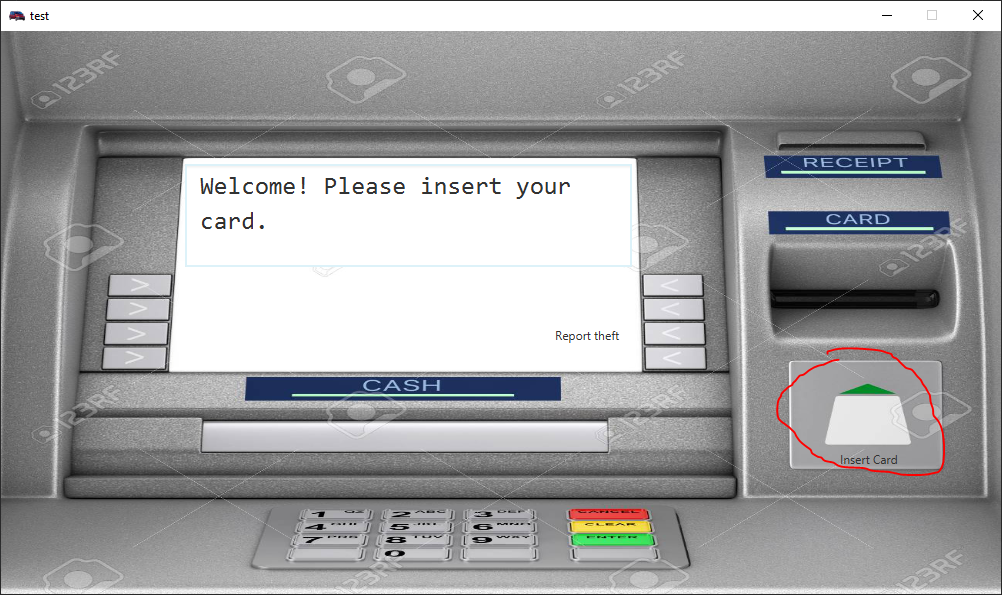
\includegraphics[width=\textwidth]{guiwithCircle.PNG}
To properly start with the program, you need to insert your card by clicking on the area highlighted by the red circle. In practice, the cursor also indicates where you can click to perform actions.\\
\subsubsection{Startup}
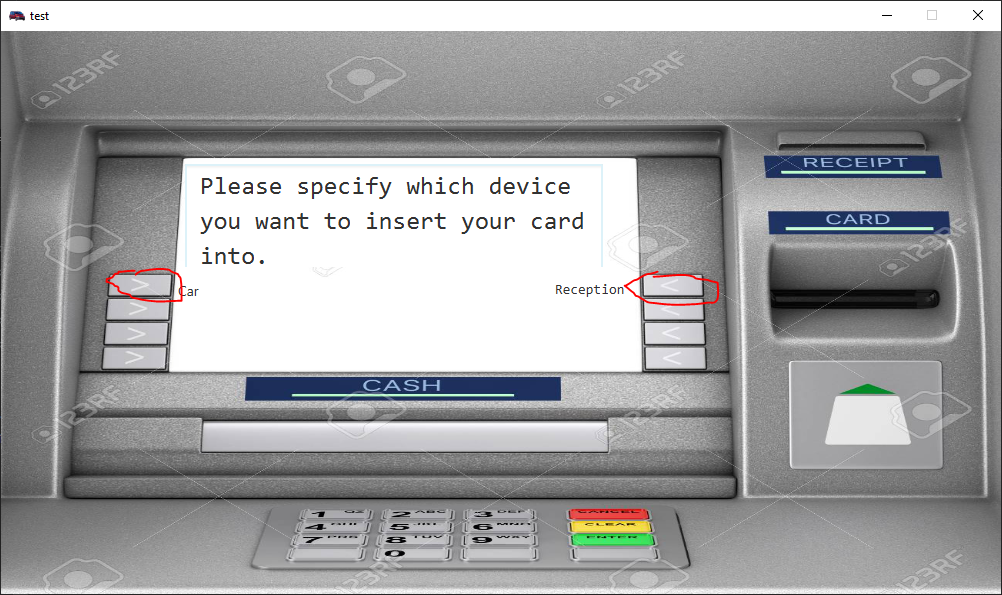
\includegraphics[width=\textwidth]{startup.PNG}
Once you insert your card, you can click on one of the highlighted buttons to indicate which terminal you would like to interact with. If you have no car assigned yet, you need to interact with the reception terminal first.
\subsubsection{Car}
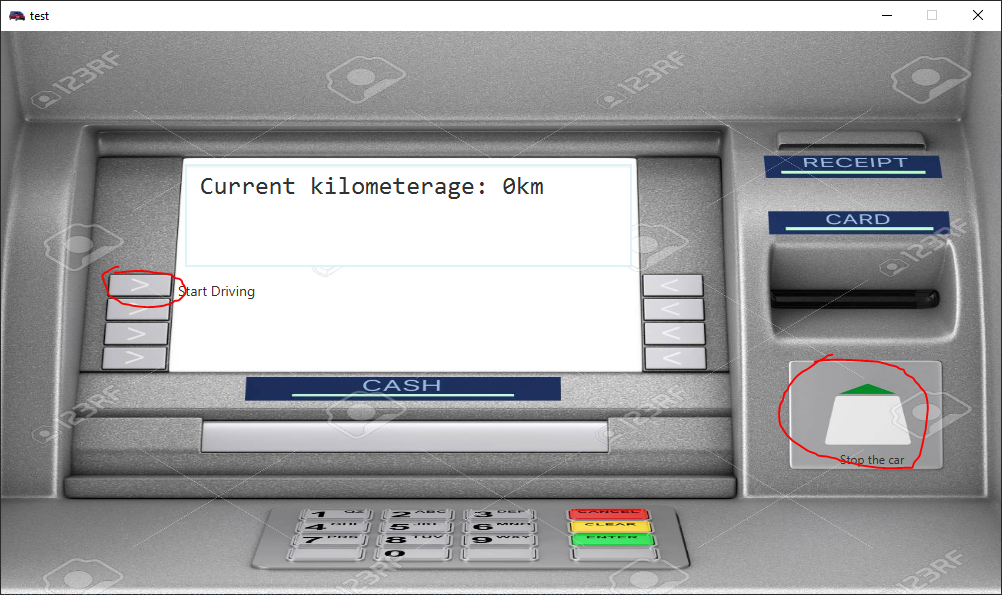
\includegraphics[width=\textwidth]{carstart.PNG}
Once you choose to start a car, you are greeted by this screen. Here you can either ignite the car or leave the car.\\\\
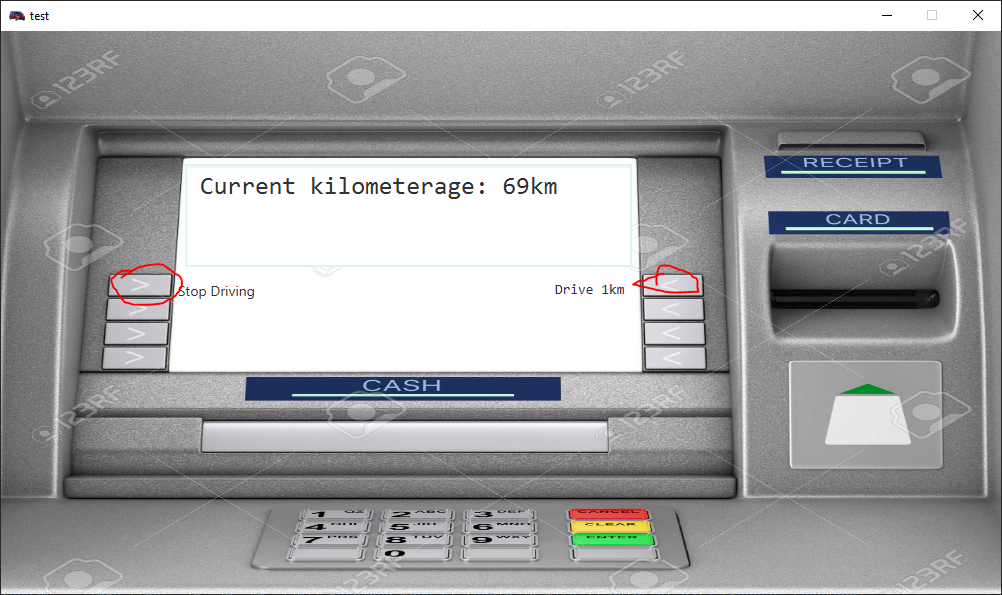
\includegraphics[width=\textwidth]{driving.PNG}
Once you start the car you can either stop the car or drive one kilometer by clicking one of the highlighted buttons. We originally wanted the program to loop here and update the kilometerage with time, however we encountered problems with \texttt{JCSystem} and multithreading, so we opted for a button instead to still be able to simulate the protocol properly.
\subsubsection{Blocking a card}
\begin{center}
    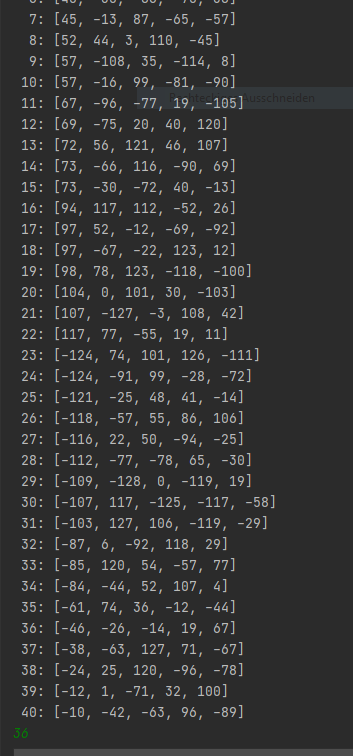
\includegraphics[scale=0.75]{cons.PNG}
\end{center}
When blocking a card, the console lists all card numbers in the database. Just enter the number of the card you want to block in the console, press enter and then hit the confirm button on the GUI. We modelled this using the console instead of a GUI interface, as in real life this process would be done by an employee. You can retrieve the card ID from the logs of previous interactions.
\end{document}

